%Fred, Mac, Yuhan NSF Grant Dec 2019
% GitHub: https://github.com/fjhickernell/NSF_CompMath2018Nov
% Overleaf: https://www.overleaf.com/9576964687whkhbmrrvhsd
\documentclass[11pt]{NSFamsart}
\usepackage{latexsym,amsfonts,amsmath,amssymb,amsthm,epsfig,extdash,multirow}
\usepackage{stackrel,tabularx,mathtools,enumitem,longtable,xspace}
\usepackage[dvipsnames]{xcolor}
\usepackage[numbers,sort&compress]{natbib}
\usepackage{hyperref,accents, booktabs}
\usepackage{algorithm, algorithmicx}
\usepackage{anyfontsize}
\usepackage{cleveref}
\usepackage{wrapfig}
\usepackage[font=small,labelfont=bf]{caption}


\voffset 0.2in
\textheight 8.8 in
\pagestyle{empty}
\pagestyle{plain}
\thispagestyle{empty}

\usepackage{minted}
\newminted{python}{frame=lines,framerule=1.5pt,breaklines=true}
\newmintinline[pyinline]{python}{}


\usepackage{algpseudocode}
\algnewcommand\algorithmicparam{\textbf{Parameters:}}
\algnewcommand\PARAM{\item[\algorithmicparam]}
\algnewcommand\algorithmicinput{\textbf{Input:}}
\algnewcommand\INPUT{\item[\algorithmicinput]}
%\algnewcommand\STATE{\item}
\algnewcommand\RETURN{\State \textbf{Return }}

%\usepackage{showlabels}
\newcommand{\Upara}[1]{\noindent{\itshape #1}:}

\newcommand{\myshade}{60}
\colorlet{mylinkcolor}{violet}
\colorlet{mycitecolor}{violet}
%\colorlet{mycitecolor}{OliveGreen}
\colorlet{myurlcolor}{YellowOrange}

\hypersetup{
	linkcolor  = mylinkcolor!\myshade!black,
	citecolor  = mycitecolor!\myshade!black,
	urlcolor   = myurlcolor!\myshade!black,
	colorlinks = true,
}


% This package prints the labels in the margin
%\usepackage[notref,notcite]{showkeys}

%\numberwithin{page} %add section before page
%\pagestyle{plain}
%\setcounter{page}{1}
%\renewcommand{\thepage}{C-\arabic{page}}

%\thispagestyle{empty} \pagestyle{empty} %to eliminate page numbers for upload
%\thispagestyle{plain} \pagestyle{plain} %to add back page numbers

\headsep-0.6in
%\headsep-0.45in

%%list of acronyms with links
\newcommand{\QMCSoft}{QMCSoft\xspace}
\newcommand{\GAIL}{GAIL\xspace}
\newcommand{\QMC}{QMC\xspace}
\newcommand{\IIDMC}{IID MC\xspace}
\newcommand{\SAMSIQMC}{SAMSI-QMC\xspace}
\newcommand{\SciPy}{SciPy\xspace}
\newcommand{\GSL}{GSL\xspace}
\newcommand{\NAG}{NAG\xspace}
\newcommand{\MATLAB}{MATLAB\xspace}
\newcommand{\Chebfun}{Chebfun\xspace}
\newcommand{\Rlang}{R\xspace}
\newcommand{\Julia}{Julia\xspace}


\textwidth6.5in
\setlength{\oddsidemargin}{0in}
\setlength{\evensidemargin}{0in}
\textheight9.0in
%\textheight9.1in

\newtheorem{theorem}{theorem}


\providecommand{\FJHickernell}{Hickernell}
\newcommand{\hf}{\widehat{f}}
\newcommand{\hg}{\widehat{g}}
\newcommand{\hI}{\hat{I}}
\newcommand{\hatf}{\hat{f}}
\newcommand{\hatg}{\hat{g}}
\newcommand{\tf}{\widetilde{f}}
\newcommand{\tbf}{\tilde{\bff}}
%\DeclareMathOperator{\Pr}{\mathbb{P}}

% Math operators
\DeclareMathOperator{\std}{std}
\DeclareMathOperator{\cost}{COST}
\DeclareMathOperator{\comp}{COMP}
\DeclareMathOperator{\loss}{loss}
\DeclareMathOperator{\lof}{lof}
\DeclareMathOperator{\reg}{reg}
\DeclareMathOperator{\CV}{CV}
\DeclareMathOperator{\size}{wd}
\DeclareMathOperator{\GP}{\mathcal{G} \! \mathcal{P}}
\DeclareMathOperator{\erf}{erf}
\DeclareMathOperator*{\argmax}{arg\,max}
\DeclareMathOperator*{\argmin}{arg\,min}
\DeclareMathOperator{\QOI}{QOI} %Quantity of Interest
\DeclareMathOperator{\POI}{POI} %Parameter of Interest
\DeclareMathOperator{\Ans}{ANS}
\DeclareMathOperator{\Var}{Var}
\DeclareMathOperator{\APP}{\widehat{\QOI}}
\DeclareMathOperator{\SURR}{SM} %surrogate model
\DeclareMathOperator{\STREND}{ST} %surrogate trend
\DeclareMathOperator{\SVAR}{SV} %surrogate variation
\DeclareMathOperator{\SVARERR}{SVU} %surrogate variation uncertainty
\newcommand{\MLS}{\textrm{MLS}\xspace} %distance weighted least squares, also known as moving least squares
%\DeclareMathOperator{\ALG}{ALG}
\DeclareMathOperator{\ERR}{ERR}
\DeclareMathOperator{\VAL}{ACQ}
\DeclareMathOperator{\OPER}{OPER}
\DeclareMathOperator{\INT}{INT}
\DeclareMathOperator{\MIN}{MIN}
\DeclareMathOperator{\ID}{ID}
\DeclareMathOperator{\APPMIN}{\widehat{\MIN}}
\DeclareMathOperator{\APPID}{\widehat{\ID}}
\DeclareMathOperator{\MINVAL}{MINACQ}
\DeclareMathOperator{\IDVAL}{IDACQ}
\DeclareMathOperator{\SURRERR}{SU}
\DeclareMathOperator{\MINERR}{MERR}
\DeclareMathOperator{\IDERR}{IDERR}
\DeclareMathOperator{\Prob}{\mathbb{P}}
\DeclareMathOperator{\diag}{diag}
\DeclareMathOperator{\dist}{dist}
\DeclareMathOperator{\filldis}{fill}
\DeclareMathOperator{\sep}{sep}
\DeclareMathOperator{\avg}{avg}
\DeclareMathOperator{\vol}{vol}
\DeclareMathOperator{\cov}{cov}
\newcommand{\TREND}{\textup{T}}
\newcommand{\VAR}{\textup{V}}
\newcommand{\LS}{\textup{LS}}







\newcommand{\reals}{{\mathbb{R}}}
\newcommand{\naturals}{{\mathbb{N}}}
\newcommand{\natzero}{{\mathbb{N}_0}}
\newcommand{\integers}{{\mathbb{Z}}}
\def\expect{{\mathbb{E}}}
\def\il{\left \langle}
\def\ir{\right \rangle}
\def\e{\varepsilon}
\def\g{\gamma}
\def\l{\lambda}
\def\b{\beta}
\def\a{\alpha}
\def\lall{\Lambda^{{\rm all}}}
\def\lstd{\Lambda^{{\rm std}}}

\newcommand{\vf}{\boldsymbol{f}}
\newcommand{\hV}{\widehat{V}}
\newcommand{\tV}{\widetilde{V}}
\newcommand{\fraku}{\mathfrak{u}}
\newcommand{\hcut}{\mathfrak{h}}
\newcommand{\tOmega}{\widetilde{\Omega}}
\newcommand{\tvarrho}{\widetilde{\varrho}}

\newcommand{\bbE}{\mathbb{E}}
\newcommand{\tQ}{\widetilde{Q}}
\newcommand{\mA}{\mathsf{A}}
\newcommand{\mB}{\mathsf{B}}
\newcommand{\mC}{\mathsf{C}}
\newcommand{\mD}{\mathsf{D}}
\newcommand{\mG}{\mathsf{G}}
\newcommand{\mH}{\mathsf{H}}
\newcommand{\mI}{\mathsf{I}}
\newcommand{\bbK}{\mathbb{K}}
\newcommand{\mK}{\mathsf{K}}
\newcommand{\tmK}{\widetilde{\mathsf{K}}}
\newcommand{\mL}{\mathsf{L}}
\newcommand{\mM}{\mathsf{M}}
\newcommand{\mP}{\mathsf{P}}
\newcommand{\mQ}{\mathsf{Q}}
\newcommand{\mR}{\mathsf{R}}
\newcommand{\mX}{\mathsf{X}}
\newcommand{\mPhi}{\mathsf{\Phi}}
\newcommand{\mPsi}{\mathsf{\Psi}}
\newcommand{\mLambda}{\mathsf{\Lambda}}
\newcommand{\cube}{[0,1]^d}
\newcommand{\design}{\{\bx_i\}_{i=1}^n}




\newcommand{\bone}{\boldsymbol{1}}
\newcommand{\bzero}{\boldsymbol{0}}
\newcommand{\binf}{\boldsymbol{\infty}}
\newcommand{\ba}{{\boldsymbol{a}}}
\newcommand{\bb}{{\boldsymbol{b}}}
\newcommand{\bc}{{\boldsymbol{c}}}
\newcommand{\bd}{{\boldsymbol{d}}}
\newcommand{\be}{{\boldsymbol{e}}}
\newcommand{\bff}{{\boldsymbol{f}}}
\newcommand{\bhh}{{\boldsymbol{h}}}
\newcommand{\beps}{{\boldsymbol{\varepsilon}}}
\newcommand{\tbeps}{\tilde{\beps}}
\newcommand{\bt}{{\boldsymbol{t}}}
\newcommand{\bT}{{\boldsymbol{T}}}
\newcommand{\bx}{{\boldsymbol{x}}}
\newcommand{\bX}{{\boldsymbol{X}}}
\newcommand{\bh}{{\boldsymbol{h}}}
\newcommand{\bj}{{\boldsymbol{j}}}
\newcommand{\bk}{{\boldsymbol{k}}}
\newcommand{\bg}{{\boldsymbol{g}}}
\newcommand{\bn}{{\boldsymbol{n}}}
\newcommand{\br}{{\boldsymbol{r}}}
\newcommand{\bv}{{\boldsymbol{v}}}
\newcommand{\bu}{{\boldsymbol{u}}}
\newcommand{\by}{{\boldsymbol{y}}}
\newcommand{\bz}{{\boldsymbol{z}}}
\newcommand{\bvarphi}{{\boldsymbol{\varphi}}}
\newcommand{\bgamma}{{\boldsymbol{\gamma}}}
\newcommand{\bphi}{{\boldsymbol{\phi}}}
\newcommand{\bpsi}{{\boldsymbol{\psi}}}
\newcommand{\btheta}{{\boldsymbol{\theta}}}
\newcommand{\bnu}{{\boldsymbol{\nu}}}
\newcommand{\balpha}{{\boldsymbol{\alpha}}}
\newcommand{\bbeta}{{\boldsymbol{\beta}}}
\newcommand{\bo}{{\boldsymbol{\omega}}}  %GF added
\newcommand{\newton}[2]{\left(\begin{array}{c} #1\\ #2\end{array}\right)}
\newcommand{\anor}[2]{\| #1\|_{\mu_{#2}}}
\newcommand{\satop}[2]{\stackrel{\scriptstyle{#1}}{\scriptstyle{#2}}}
\newcommand{\setu}{{\mathfrak{u}}}

\newcommand{\me}{\textup{e}}
\newcommand{\mi}{\textup{i}}
\def\d{\textup{d}}
\def\dif{\textup{d}}
\newcommand{\cc}{\mathcal{C}}
\newcommand{\cb}{\mathcal{B}}
\newcommand{\cl}{L}
\newcommand{\ct}{\mathfrak{T}}
\newcommand{\cx}{{\Omega}}
\newcommand{\cala}{{\mathcal{A}}}
\newcommand{\calc}{{\mathcal{C}}}
\newcommand{\calf}{{\mathcal{F}}}
\newcommand{\calfd}{{\calf_d}}
\newcommand{\calh}{{\mathcal{H}}}
\newcommand{\tcalh}{{\widetilde{\calh}}}
\newcommand{\calI}{{\mathcal{I}}}
\newcommand{\calhk}{\calh_d(K)}
\newcommand{\calg}{{\mathcal{G}}}
\newcommand{\calgd}{{\calg_d}}
\newcommand{\caln}{{\mathcal{N}}}
\newcommand{\calp}{{\mathcal{P}}}
\newcommand{\cals}{{\mathcal{S}}}
\newcommand{\calu}{{\mathcal{U}}}
\newcommand{\cL}{\mathcal{L}}
\newcommand{\cP}{\mathcal{P}}
\newcommand{\cT}{\mathcal{T}}
\newcommand{\cK}{\mathcal{K}}
\newcommand{\fA}{\mathfrak{A}}
\newcommand{\fC}{\mathfrak{C}}
\newcommand{\fF}{\mathfrak{F}}
\newcommand{\fL}{\mathfrak{L}}
\newcommand{\fU}{\mathfrak{U}}
\newcommand{\hS}{\widehat{S}}

\def\abs#1{\ensuremath{\left \lvert #1 \right \rvert}}
\newcommand{\bigabs}[1]{\ensuremath{\bigl \lvert #1 \bigr \rvert}}
\newcommand{\norm}[2][{}]{\ensuremath{\left \lVert #2 \right \rVert}_{#1}}
\newcommand{\ip}[3][{}]{\ensuremath{\left \langle #2, #3 \right \rangle_{#1}}}
\newcommand{\bignorm}[2][{}]{\ensuremath{\bigl \lVert #2 \bigr \rVert}_{#1}}
\newcommand{\Bignorm}[2][{}]{\ensuremath{\Bigl \lVert #2 \Bigr \rVert}_{#1}}
\newcommand{\calm}{{\mathfrak{M}}}

\newcommand{\des}{\{\bx_i\}}
\newcommand{\desinf}{\{\bx_i\}_{i=1}^{\infty}}
\newcommand{\desn}{\{\bx_i\}_{i=1}^n}
\newcommand{\wts}{\{g_i\}_{i=1}^N}
\newcommand{\wtsn}{\{g_i\}_{i=1}^N}
\newcommand{\datan}{\{y_i\}_{i=1}^N}

%FJH added
\newcommand{\Order}{\mathcal{O}}
\newcommand{\ch}{\mathcal{H}}
\newcommand{\tch}{{\widetilde{\ch}}}
\newcommand{\veps}{\boldsymbol{\varepsilon}}
\DeclareMathOperator{\best}{best}
\newcommand{\hmu}{\hat{\mu}}
\newcommand{\hsigma}{\hat{\sigma}}
\newcommand{\tK}{\widetilde{K}}
%\newcommand{\Matlab}{{\sc Matlab}\xspace}
\newcommand{\abstol}{\varepsilon_{\text{a}}}
\newcommand{\reltol}{\varepsilon_{\text{r}}}

\newcommand\starred[1]{\accentset{\star}{#1}}

\newcommand{\designInf}{\{\bx_i\}_{i=1}^\infty}
\newcommand{\dataN}{\bigl\{\bigl(\bx_i,f(\bx_i)\bigr)\bigr\}_{i=1}^n}
\newcommand{\dataNp}{\bigl\{\bigl(\bx_i,f(\bx_i)\bigr)\bigr\}_{i=1}^{n'}}
\newcommand{\dataNo}{\bigl\{\bigl(\bx_i,f(\bx_i)\bigr)\bigr\}_{i=1}^{n_0}}
\newcommand{\ErrN}{\ERR\bigl(\dataN,n\bigr)}
\newcommand{\fint}{f_{\text{int}}}
\newcommand{\inflate}{\fC}
\newcommand{\IIDSim}{\overset{\text{IID}}{\sim}}
\newcommand{\LDSim}{\overset{\text{LD}}{\sim}}


\definecolor{MATLABOrange}{rgb}{0.85,  0.325, 0.098}


%\setcounter{page}{1}


\setlist[description]{font=\normalfont\itshape, labelindent = 0.5cm}
\setlist[itemize]{leftmargin=5ex}

\makeatletter
\newenvironment{varsubequations}[1]
 {%
  \addtocounter{equation}{-1}%
  \begin{subequations}
  \renewcommand{\theparentequation}{#1}%
  \def\@currentlabel{#1}%
 }
 {%
  \end{subequations}\ignorespacesafterend
 }
\makeatother


\newcommand{\FJHNote}[1]{{\color{blue}Fred: #1}}
\newcommand{\JMHNote}[1]{{\color{green}Mac: #1}}

% Notes on the paper for communicating with coauthors
\newif\ifnotesw \noteswtrue
\newcommand{\notes}[1]{\ifnotesw \textcolor{red}{  $\clubsuit$\ {\sf \bf \it  #1}\ $\clubsuit$  }\fi}
%\noteswfalse   % comment this line out to turn on style notes 
\begin{document}
%\setlength{\leftmargini}{2.5ex}

\begin{center}
\Large \textbf{
QMCPy: Quasi-Monte Carlo Community Software\\ 
%Project Description
}
\end{center}
\vspace{-2ex}

\setcounter{tocdepth}{1}
\tableofcontents

\vspace{-6ex}


Quasi-Monte Carlo (QMC) methods replace independent and identically distributed (IID) points by low discrepancy (LD) points to improve efficiency.  We, Fred Hickernell (FH, PI from Illinois Tech), Simon Mak (SM, PI from Duke U), and Sou-Cheng Terrya Choi (SCTC, Senior Personnel) propose to grow QMCPy \cite{QMCPy2020a}, a Python QMC software library, which will be embraced by the community of QMC researchers and benefit an expanding base of QMC users.  QMCPy will become
\begin{enumerate}
\renewcommand{\labelenumi}{\arabic{enumi}.}
    \item A tightly-connected collection of the best QMC software, including
    \begin{enumerate}
    \renewcommand{\labelenumii}{\alph{enumii}.}
        \item LD sequence generators,
        \item QMC algorithms, such as multi-level algorithms, automatic stopping criteria, and variance/variation reduction, and
        \item Illuminating use cases,
    \end{enumerate}
    \item A user-friendly, consistent interface to the contributions of many,
    \item A proving ground for new QMC ideas,
    \item Owned and cultivated by our QMC community, and
    \item An easy on-ramp for those who are new to QMC.
\end{enumerate}

Here we provide an overview of QMC, a description of our early efforts, our plans to grow QMCPy, the benefits of QMCPy, and why ours is the right team for this project.

\section{Overview of QMC and LD Sampling}

\subsection{Applications of (Q)MC}  Many situations are best understood by building randomness into the mathematical model.  Examples include Bayesian statistical inference \cite{}, financial risk \cite{Gla03}, photon transport \cite{}, and uncertainty quantification \cite{}.  Simulations use random vectors to generate a myriad of possible outcomes.  The statistical properties of these sample outcomes---such as means (averages), quantiles, and probability densities---can effectively estimate the population quantities.  This is the (Q)MC process:  IID sampling for simple MC and LD sampling for QMC.

Cubatures for approximating multivariate integrals based on grid sampling have computational costs that increase exponentially with the number of variables, $d$.  (Q)MC simulation avoids this curse of dimensionality with computational costs that are often only weakly dimension dependent.

In constructing surrogate models for computer experiments (multivariate function approximation), one may wish to evenly sample the domain to search for regions where the function changes more sharply.  IID and LD sampling again prove advantageous over grid sampling.

\subsection{LD Versus IID Sampling} \label{sec:LDvsIID}

The quantity of interest, $Y$ (option payoff, pixel intensity, pressure at certain location), is commonly expressed as a function of a $d$-dimensional vector random variable $\bX$, i.e., $Y = f(\bX)$.  We assume that $\bX$ follows a cumulative distribution function $F:\cx \subseteq \reals^d \to [0,1]$.  When $f$ has a complicated form, the population mean (multivariate integral), $\mu$, cannot be computed analytically.  But, it may be estimated the sample mean:
\begin{equation} \label{eq:mean}
    \mu = \bbE(Y) = \int_{\cx} f(\bx) \, \dif F(\bx) \approx
\hmu_n = \frac 1n \sum_{i=1}^n Y_i = \frac 1n  \sum_{i=1}^n f(\bX_i).
\end{equation}
How should $\bX_1, \bX_2, \ldots $ be chosen to make $\abs{\mu - \hmu_n} \le \varepsilon$?

Fig.\ \ref{fig:iid_vs_ld} displays $n=64$ IID, LD, and grid points intended to mimic $\calu[0,1]^2$, the standard uniform distribution in dimension $d=2$.  The points on the left, $\bX_1, \bX_2,  \ldots \IIDSim \calu[0,1]^2$, are random and do not know about each other.  Since these points are IID, the multivariate distribution of $\bX_1, \ldots \bX_n$ is a product of the bivariate marginals:  $F_{n}(\bx_1, \ldots, \bx_n) = F(\bx_1) 
\cdots F(\bx_n) = x_{11}x_{12} x_{21} \cdots x_{n2}$, where $F(\bx)  = x_1x_2$ is the bivariate uniform distribution.

\begin{figure}[H]
	\centering
	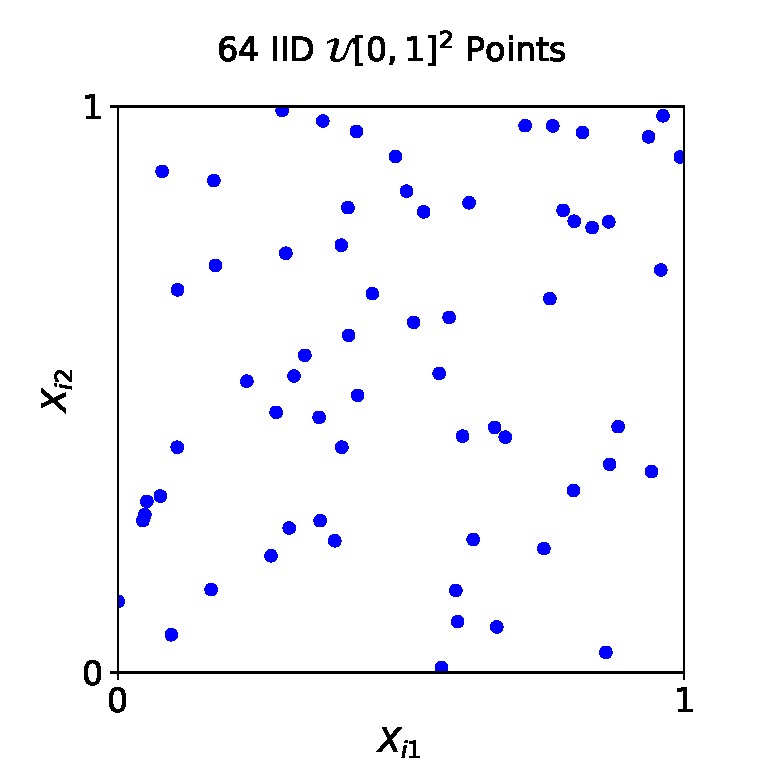
\includegraphics[height = 5cm]{ProgramsImages/iid_scatter.eps} \quad
	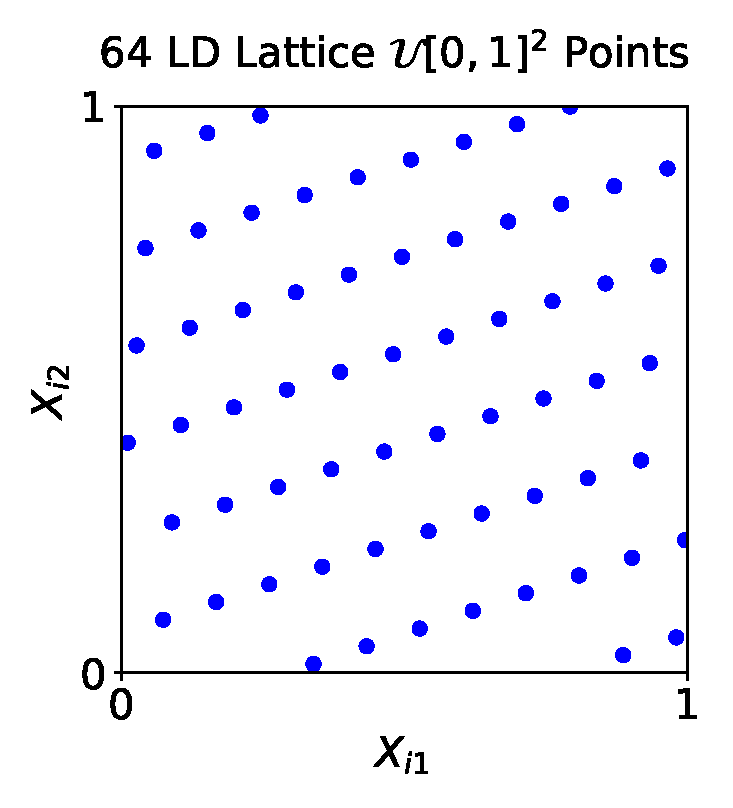
\includegraphics[height = 5cm]{ProgramsImages/lattice_scatter.eps} \quad
	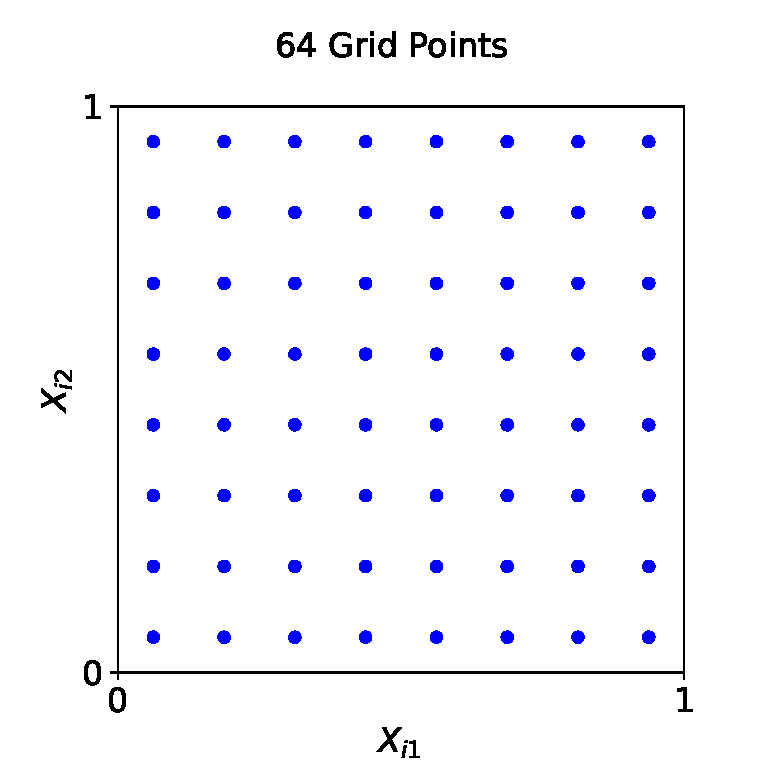
\includegraphics[height = 5cm]{ProgramsImages/grid_scatter.eps}
	\caption{IID points (left), LD lattice points (center), and grid points (right).  The LD points have fewer gaps and clusters of points that either the IID or grid points. \label{fig:iid_vs_ld}}
\end{figure}

The  points in the center of Fig.\ \ref{fig:iid_vs_ld}, $\bX_1, \bX_2,  \ldots \LDSim \calu[0,1]^2$, are carefully coordinated with one another.  They might be deterministic or random.  They are designed to mimic the distribution $F$  in the sense that the empirical distribution function of  $\bX_1, \ldots \bX_n$---denoted $F_{\{\bX_i\}_{i=1}^n}$---is close to $F$.  (The empirical distribution for $n$  points assigns probability $1/n$ to each of point.)  A \emph{discrepancy}, $D(\{\bX_i\}_{i=1}^n, F)$, measures the size of $F - F_{\{\bX_i\}_{i=1}^n}$, and LD points make the discrepancy small.  Discrepancies are explained further in the next subsection and in Sect. \ref{}.

The points on the right in Fig.\ \ref{fig:iid_vs_ld} are grid points. While they may look even, they lack evenness in low dimensional projections.  Specifically, the grid points have only $\sqrt{n} = 8$ equally spaced values in each coordinate direction, whereas the LD points have $n=64$ equally spaced values.  For $d$-dimensional grids, there are only $n^{1/d}$ values in each coordinate direction, which is disastrous for  large $d$.

\subsection{Efficiency Benefits from LD Sampling}
The root mean squared error of the sample mean, $\hmu_n$ in approximating the population mean, $\mu$, when IID samples are used is 
\begin{equation}
    \sqrt{\bbE\bigl[\abs{\mu - \hmu_n}^2\bigr]} = \frac{\std(Y)}{\sqrt{n}},  \quad \std(Y) = \sqrt{\int_{\cx} \abs{f(\bx) - \mu}^2 \, \dif F(\bx)}, \qquad \bX_1, \bX_2, \ldots \text{IID}.
\end{equation}
The smoothness requirement on $f$ is minimal, and the error bound is free from the curse of dimensionality (assuming that $\std(Y)$ does not explode with dimension), but the convergence rate is modest.  

For LD sampling the absolute error has an upper bound of
\begin{equation}
    \abs{\mu - \hmu_n}^2 \le D(\{\bX_i\}_{i=1}^n, F) \norm[\calf]{f},  \qquad \bX_1, \bX_2, \ldots \text{LD}.
\end{equation}
The Banach space $\calf$ typically requires somewhat more smoothness than the $L^2$ requirement for IID sampling, e.g., $L^2$ mixed partial derivatives of up to order one in each coordinate direction. The discrepancy,  $D(\{\bX_i\}_{i=1}^n, F)$, corresponds to the norm of the cubature error functional \cite{Hic97a}, and is typically $\Order(n^{-1 + \delta})$ for well-chosen LD sequences, where $\delta$ is arbitrarily small and positive.

Fig.\ \ref{fig:KeisterTimes} displays the results of approximating an integral from a computational physics example of Keister \cite{Kei96},
\begin{equation} \label{eq:Keister}
\mu = \int_{\reals^d} \cos( \norm[2]{\bt}) \exp(-\norm[2]{\bt}^2) \, \dif \bt,
\end{equation}
for the case $d =5$ under several absolute error tolerances, $\varepsilon$, using QMCPy.  Both the number of function values and the computation time increase like $\Order(\varepsilon^{-2})$ for IID sampling and $\Order(\varepsilon^{-1-\delta})$ for LD sampling as $\varepsilon$ decreases. 


\begin{wrapfigure}{r}{0.75\textwidth}
	\centering
	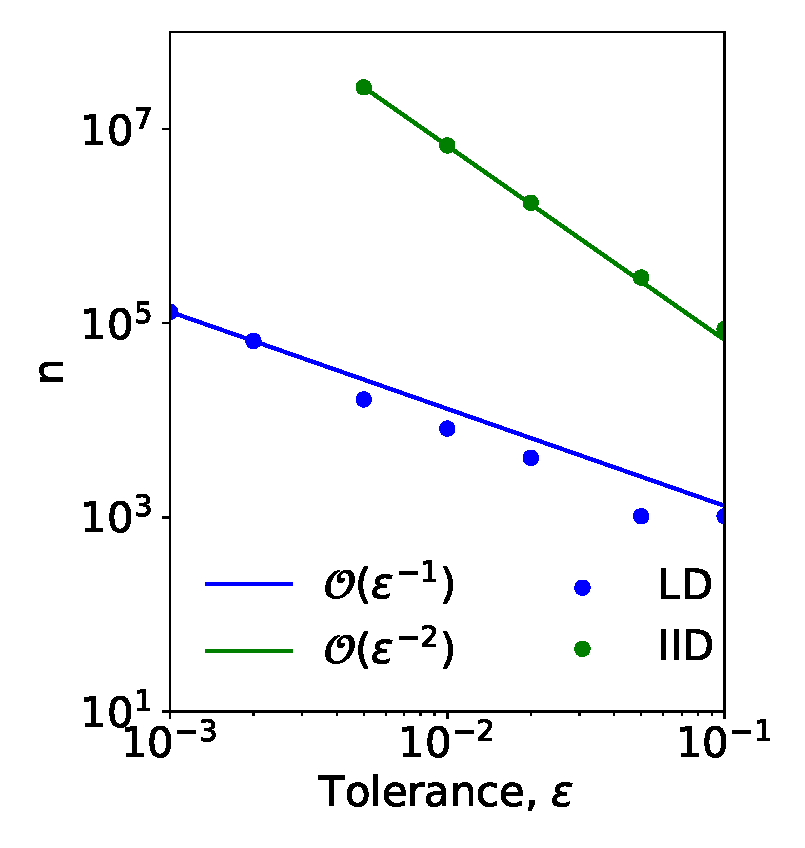
\includegraphics[height =0.35\textwidth]{ProgramsImages/keister_n.eps}
	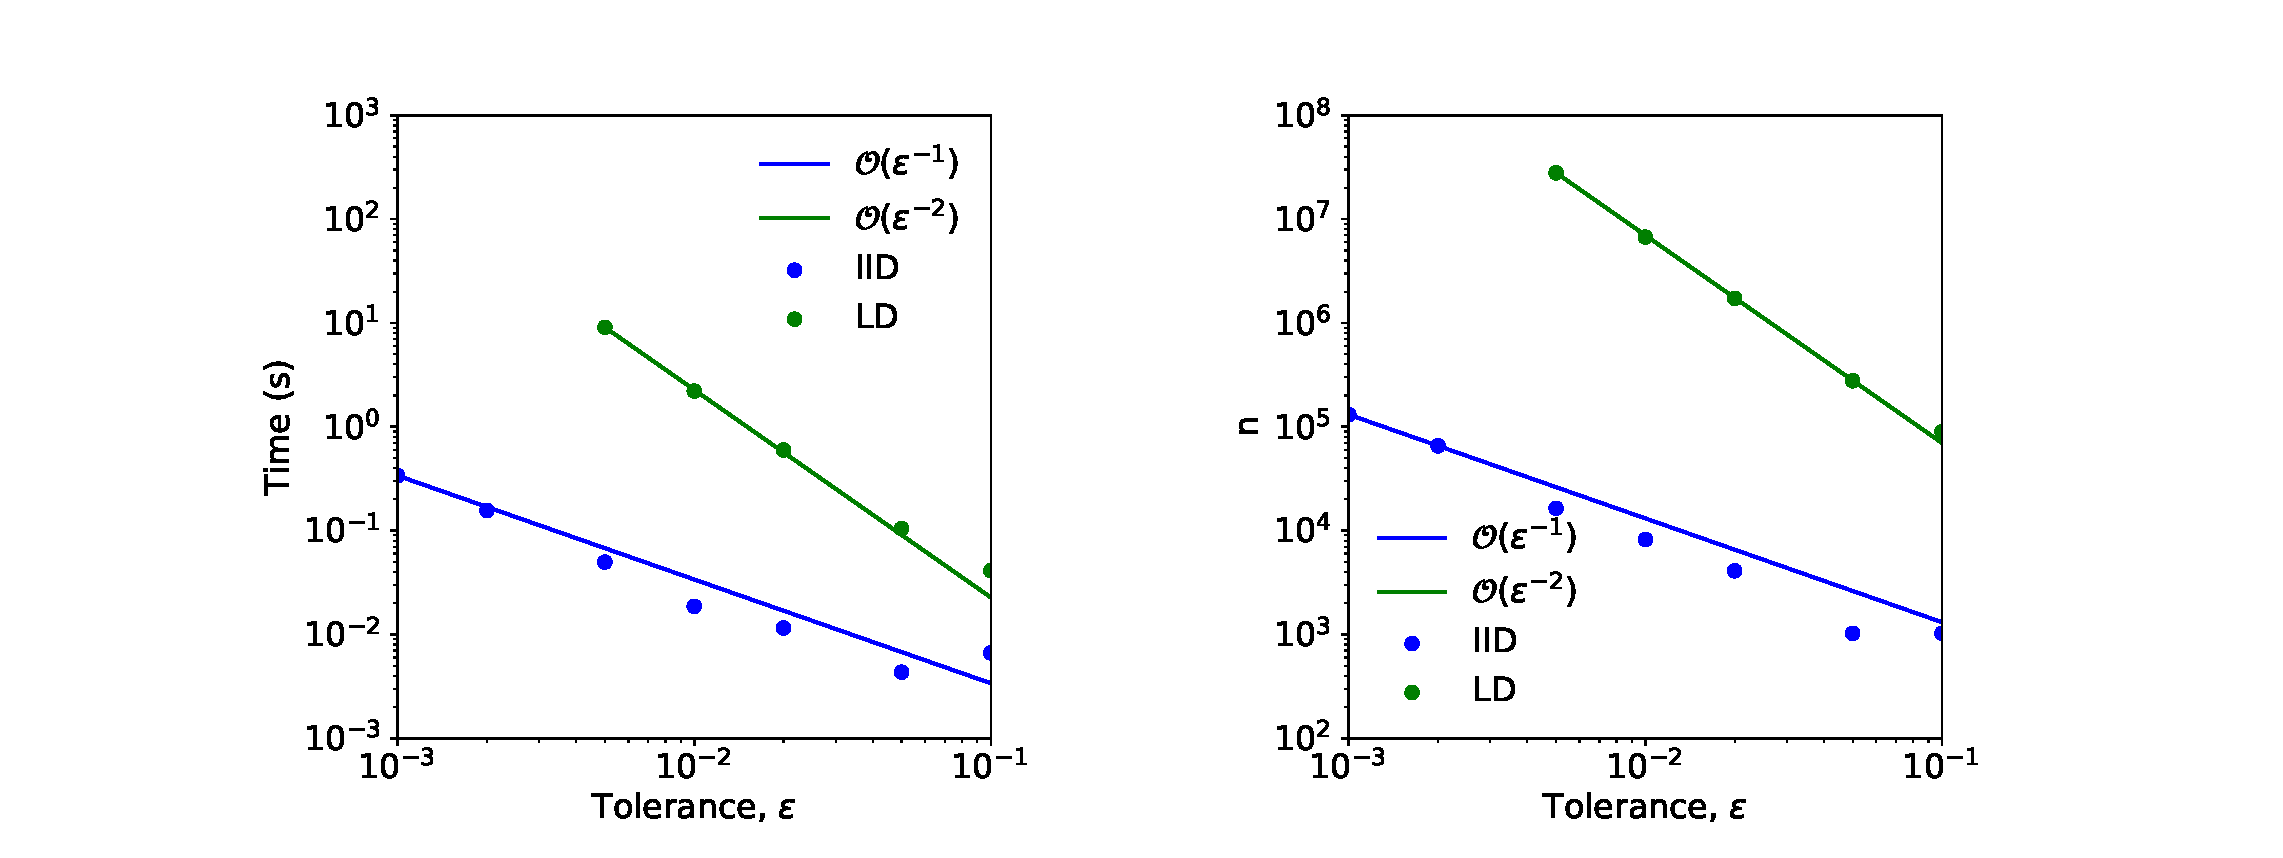
\includegraphics[height =0.35\textwidth]{ProgramsImages/keister_timing.eps} 
	\caption{Number of function values (left) and run time (right) required to compute the Keister integral \eqref{eq:Keister} using QMCPy.  LD sampling is substantially more efficient than IID sampling, especially as the error tolerance decreases.}
	\label{fig:KeisterTimes}
\end{wrapfigure}



The advantage of LD sampling is illustrated by the sharp divergence of the times and function values required as $\varepsilon$ decreases.  For $\varepsilon = 0.01$ there is already a marked contrast between tens of thousands of function values and hundredths of seconds for LD versus millions of function values and seconds for IID.

The computational cost rates of increase as $\varepsilon$ decreases for IID and LD sampling are essentially \emph{independent of $d$}.  This is not the case for tensor product rules.  If the derivatives of $f$ up to total order $rd$ exist, then there exist tensor product rules that provide $\abs{\mu - \hmu_n} \le \varepsilon$  at a cost (time or function values) of $\Order(\varepsilon^{-d/r})$.  While increased smoothness, $r$, helps, it cannot overcome the curse of dimensionality, i.e., exponential growth of the cost with $d$.

To harness the efficiency of LD sampling via QMC methods, practitioners need quality software that is easy to use.  QMC researchers need a proving ground for their latest developments.  This is why we need QMCPy.

\section{QMCPy Now}

\subsection{The Start of QMCPy}
During the summer of 2018 Fred Hickernell (FH) began discussing with other QMC researchers, including Dirk Nuyens, Frances Kuo, and Art Owen (AO) how we could combine our software efforts into a community owned library.  The better existing QMC software efforts now and then include the following:
\begin{description}[format=\textup]
	\item[MATLAB] Sobol' and Halton sequences in their Statistics and Machine Learning Toolbox, commercial \cite{MAT9.8}
	\item [qrng]  Sobol' and Halton sequences in R \cite{QRNG2020}
	\item[BRODA] Sobol' sequences in C, MATLAB, and Excel \cite{BRODA20a}
	\item[PyTorch] Scrambled Sobol' sequences \cite{PyTorch}
	\item[LatNet Builder] Generating vectors/matrices for lattices and digital nets \cite{LatNet}
	\item[MPS] Magic Point Shop, lattices and Sobol' sequences \cite{Nuy17a}
	\item[Owen] Randomized Halton sequences in R \cite{Owe20a}
	\item[Robbe] LD Sequences in Julia \cite{Rob20a}
	\item[Burkhardt] various QMC software in C++, Fortran, MATLAB, \& Python \cite{Bur20a}
	\item[SSJ] Stochastic Simulation in Java \cite{SSJ}
	\item[ML(Q)MC] Multi-Level (Quasi-)Monte Carlo routines in C++, MATLAB, Python, and R \cite{GilesSoft}
	\item[QMC4PDE] QMC for elliptic PDEs with random diffusion coefficients \cite{KuoNuy16a}
	\item[GAIL] Automatic stopping criteria for (Q)MC in MATLAB \cite{ChoEtal20a}
	\item[UQLab] Framework for Uncertainty Quantification in MATLAB \cite{UQLab2014}
	\item[OpenTURNS] Open source initiative for the Treatment of Uncertainties, Risks 'N Statistics in Python \cite{OpenTURNS}
\end{description}
Each of these software packages focus on just certain aspects of QMC: some packages focus on the generation of LD sequences, some packages focus on fundamental QMC algorithms, and other packages focus on particular applications of QMC.  The software packages listed above are primarily the initiatives of individual research groups, not a shared community effort.

Fruitful discussions in 2018 that carried into further discussions with Mike McCourt (MM) in early 2019.  MM's company, Silicon Valley startup SigOpt, offered to fund the early stage development of  QMCPy, which would combine the efforts of several different research groups into a cutting edge package. Python 3 was chosen as the language based on its popularity among a broad sector of potential users, especially those in the high tech industry.  Also, Python supports C libraries to speed up crucial code.  Aleksei Sorokin (AS),  a co-terminal BS applied mathematics and MS data science student at Illinois Tech, was hired to do create the QMCPy code.  QMCPy was released in the summer of 2020.  QMCPy may be installed using \pyinline{pip} and imported via \pyinline{from qmcpy import *}.

FH gave a tutorial on QMC software---with a focus on QMCPy---at MCQMC 2020 \cite{MCQMC2020QMCPyTut}.  A Google Colaboratory notebook \cite{QMCPyTut2020} was made available for the audience to try QMCPy simultaneously with the tutorial.  FH, SCTC, AO, AS, and MM wrote a series of blogs \cite{QMCBlog} to introduce QMC to the broader community to QMC.



\subsection{QMCPy Architecture}

Arising from the aforementioned discussions, it was decided that QMCPy should have four major abstract classes:
\begin{itemize}
	\item \pyinline{DiscreteDistribution} for generating LD and IID sequences according to their original probability distributions,
	\item \pyinline{TrueMeasure} to accommodate problems defined for more general distributions or measures,
	\item \pyinline{Integrand} to define the particular function, $f$, of interest, and
	\item \pyinline{StippingCriterion} to determine when to stop the simulation.
\end{itemize}
There is also an \pyinline{AccumulateData} class to keep track of intermediate results.

\subsubsection{\textup{\pyinline{DiscreteDistribution} and \pyinline{TrueMeasure}}} LD sequences are constructed by creating the object and then generating the points.  The code below illustrates how to generate the points shown in the center panel of Fig.\ \ref{fig:iid_vs_ld}.
\begin{pythoncode}
ld = qmcpy.Lattice(dimension = 2)  #define a discrete LD distribution 
points = lattice.gen_samples(n = 64)  #construct points
\end{pythoncode}

All LD generators provide points designed to mimic the distribution $\calu[0,1]^d$.  QMCPy also has \pyinline{Sobol} \cite{DicPil10a} and \pyinline{Halton} \cite{Hal60} LD generators whose syntax are comparable.  Fig.\ \ref{fig:sobol_halton} illustrates these LD points.  For comparison purposes, QMCPy also has standard uniform and normal psuedo-random generators adapted from \pyinline{numpy}.  
 
Our LD generators are extensible, meaning that one may generate additional points while reusing the ones that have already been generated.  For lattice and Sobol' points it is preferable that $n$ be a power of $2$, while Halton points have no preferred $n$, but may have a somewhat larger in discrepancy than the others.
 
\iffalse
\begin{wrapfigure}{r}{0.65\textwidth}
	\centering
	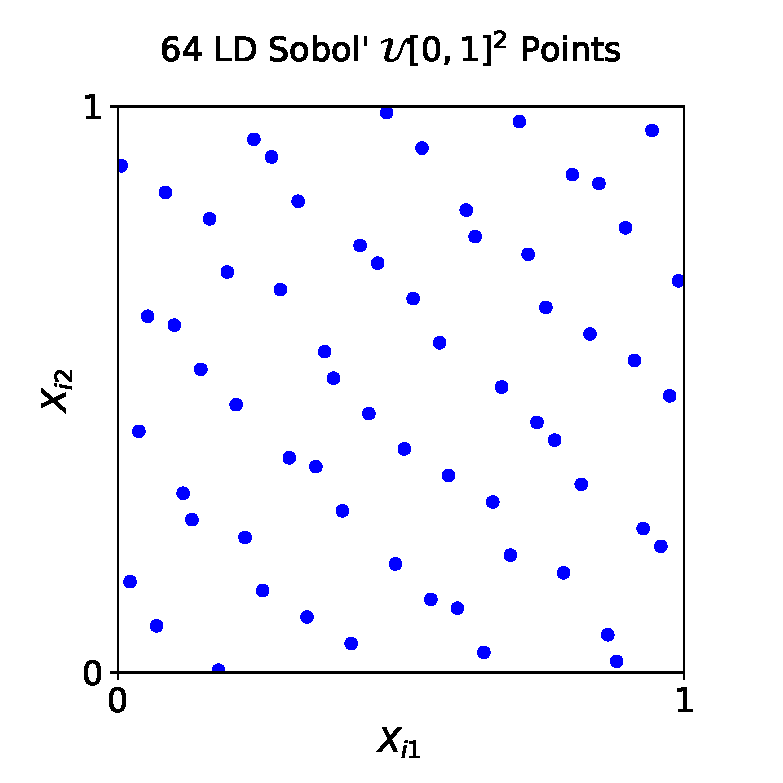
\includegraphics[height = 5cm]{ProgramsImages/sobol_scatter.eps} 
	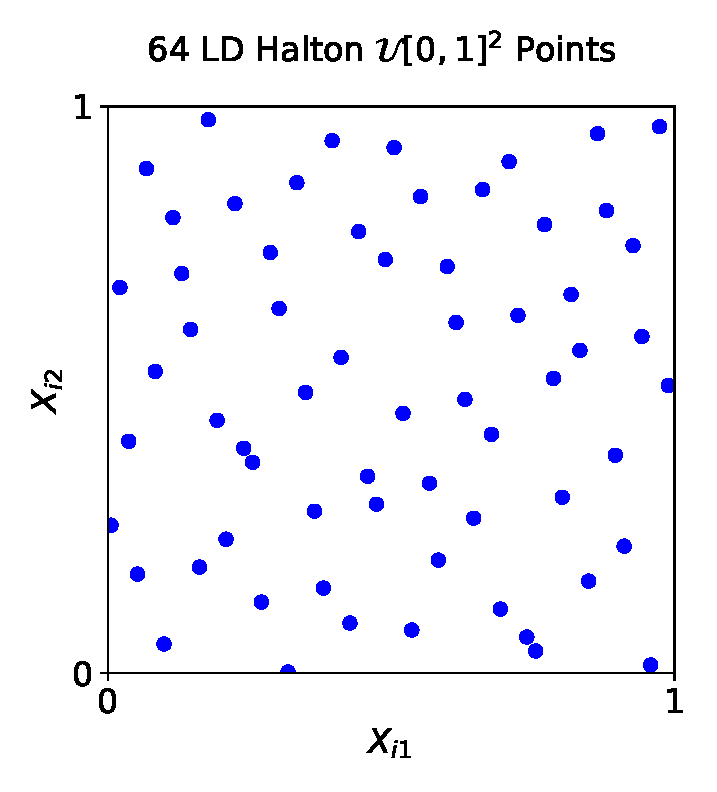
\includegraphics[height = 5cm]{ProgramsImages/halton_scatter.eps}
	\caption{LD Sobol' (left) and Halton points (right).  These points also have fewer gaps and clusters than IID points. \label{fig:sobol_halton}}
\end{wrapfigure}
\fi
All QMCPy LD generators are randomized by default to ensure that no points lie on the boundary of the unit cube.  This means that if points are transformed to mimic the Gaussian or other distributions on $\reals^d$, no LD points will be mapped to infinity.  Randomizing Sobol' points can improve the rate of convergence of $\hmu_n$ to $\mu$ \cite{Owe97}.

To construct good points that mimic distributions other than standard uniform, one must transform the original points.  The  inverse cumulative distribution if often used.  The \pyinline{TrueMeasure} class automates that transformation.
\begin{pythoncode}
gaussian_ld = qmcpy.Gaussian(qmcpy.Lattice(2), mean = [3,2], covariance = [[9,5],[5,4]])  #specify the distribution parameters 
points = gaussian_ld.gen_samples(n = 64)  #construct points
\end{pythoncode}


\begin{wrapfigure}{r}{0.65\textwidth}
	\centering
	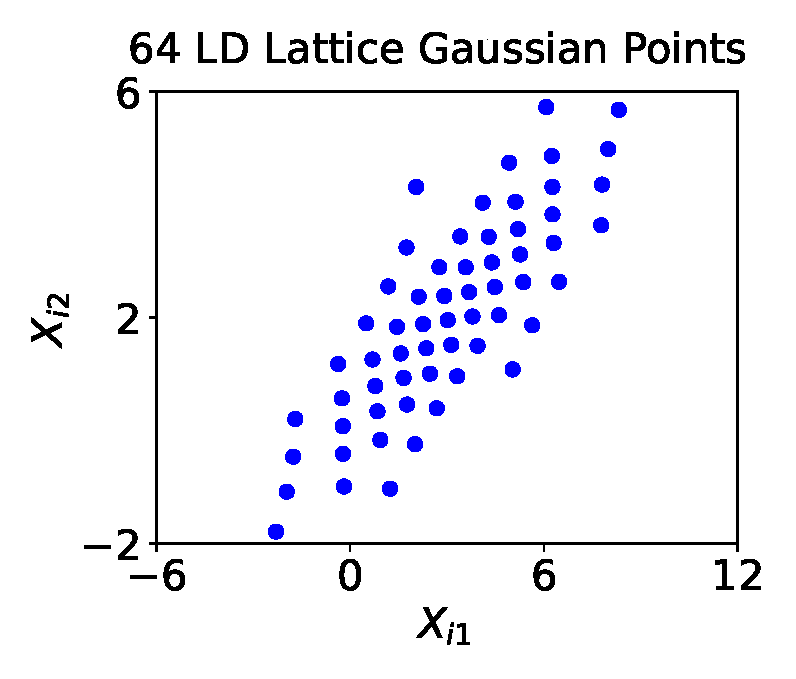
\includegraphics[height = 4.2cm]{ProgramsImages/Gauss_lattice.eps} 
	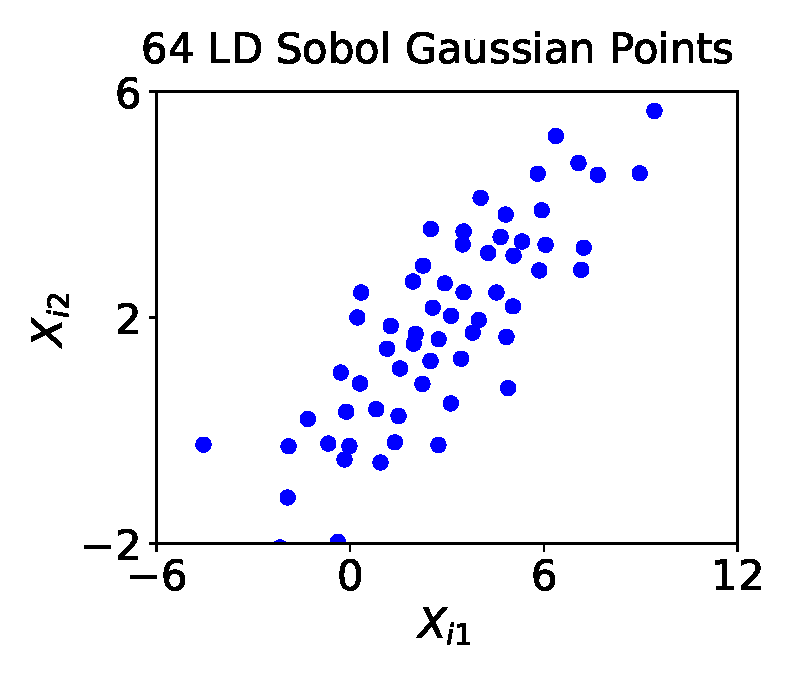
\includegraphics[height = 4.2cm]{ProgramsImages/Gauss_Sobol.eps}
	\caption{LD lattice (left) and Sobol'  (right) points transformed to mimic a Gaussian distribution.  They have a more regular structure than IID points. \label{fig:ld_Gauss}}
\end{wrapfigure}

Fig.\ \ref{fig:ld_Gauss} displays  lattice and Sobol' points that have been transformed to mimic the Gaussian distribution with mean $\begin{pmatrix} 3 \\ 2 \end{pmatrix}$ and covariance matrix $\begin{pmatrix} 9 & 5 \\ 5 & 4 \end{pmatrix}$.  A set of transformed low discrepancy points may or may not be low discrepancy with respect to the new distribution, depending on how one defines the discrepancy \cite{LiKanHic20a}.  But, transformed low discrepancy points often outperform IID points in Monte Carlo calculations.

\subsubsection{\textup{\pyinline{Integrand} and \pyinline{StoppingCriterion}}} 
For computing expectations and multivariate integration as described in \eqref{eq:mean}, one must specify the integrand.  Sometimes original form of the problem is not convenient for computation.  For example, the Keister integral in \eqref{eq:Keister} can be thought of as an integral of $g$ with respect to the Gaussian distribution with independent marginals of zero mean and variance $1/2$:
\begin{multline} \label{eq:KeisterAlt}
\mu = \int_{\reals^d} \underbrace{\pi^{d/2} \cos( \norm[2]{\bt})}_{g(\bt)}  \, \underbrace{\pi^{-d/2}\exp(-\norm[2]{\bt}^2)\, \dif \bt}_{\caln(\bzero, \mI/2)} 
= \int_{\reals^d} \underbrace{\cos( \norm[2]{\bt}) \exp(-\norm[2]{\bt}^2)}_{h(\bt)}  \, \underbrace{\dif \bt}_{\text{Lebesgue}} \\
=   \int_{[0,1]^d} f(\bx) \, \dif \bx \qquad \text{for an appropriate transformation } \bt = \bT(\bx).
\end{multline}
Alternatively, $\mu$ can be thought of as an integral of $h$ with respect to Lebesgue measure.  QMCPy can compute the integral either way.

The first way begins by constructing the Gaussian transformed LD \pyinline{TrueMeasure} instance \pyinline{gs} as discussed in the previous section.  Next, one defines the function $g$ as in \eqref{eq:KeisterAlt} above, and then uses \pyinline{CustomFun} to construct an integrand $f$ for which the integral can be written in terms of the uniform distribution, which the LD sequence mimics.  The statement below involving \pyinline{CustomFun} constructs the transformation $\bT$ in \eqref{eq:KeisterAlt}.
\begin{pythoncode}
gs = qmcpy.Gaussian(qmcpy.Sobol(5), covariance = 1/2)    #choose the Gaussian distribution
def g(t):  #your desired integrand, calculations must be vectorized
	d = t.shape[1]
	g_val = np.pi**(d/2) * np.cos(np.sqrt((t**2).sum(1))) 
	return g_val  #size n vector
f = qmcpy.CustomFun(gs, custom_fun = g)
sc = qmcpy.CubQMCSobolG(f, abs_tol = 1e-3)   #stopping criterion must match  points
solution = sc.integrate()
\end{pythoncode}

The final stage of the computation requires the construction of a \pyinline{StoppingCriterion} instance, \pyinline{sc}.  The one here is from \cite{HicJim16a} and is based on Walsh transformations of the sampled integrand data.  Invoking the \pyinline{integrate} method of \pyinline{sc} yields $\hmu_n$ satisfying
\begin{equation} \label{eq:error_crit}
	\abs{\mu -\hmu_n} \le \varepsilon,
\end{equation}
where $\varepsilon$ is the absolute error tolerance.

Another way to compute the Keister integral, \eqref{eq:Keister}, is to think of it as an integral with respect to the Lebesgue mesaure.  Again \pyinline{CustomFun} makes the proper variable transformation, and the answer is the same as the first way.  This second way takes about half the time as the first way.

 \begin{pythoncode}
lb = qmcpy.Lebesgue(qmcpy.Sobol(5), lower_bound=-np.inf, upper_bound=np.inf)   #choose the Lebesgue distribution
def h(t):  #your desired integrand, calculations must be vectorized
 	norm = np.sqrt((t**2).sum(1))  #
 	h_val = np.cos(norm) * np.exp(-norm**2)
 	return h_val  #size n vector
 f = qmcpy.CustomFun(lebesgue, custom_fun = h)
 sc = qmcpy.CubQMCSobolG(f, abs_tol = 1e-3)  #stopping criterion must match  points
 solution = sc.integrate()
 \end{pythoncode}
 
 \subsection{QMCPy Options}
 QMCPy has several options for users:
 \begin{itemize}
 	\item Backends for \pyinline{Sobol} from PyTorch \cite{PyTorch} and MPS \cite{Nuy17a}, in addition to the default from \pyinline{qrng} \cite{QRNG2020};
 	
 	\item Backends for \pyinline{Lattice} from MPS \cite{Nuy17a}, in addition to the default from GAIL \cite{ChoEtal20a}, and generating vectors from LatNet Builder \cite{LatNet};
 	
 	\item Stopping criteria based on the Central Limit Theorem (CLT) for IID sampling and random replications of LD sampling;  a more rigorous stopping criterion for IID sampling based on a Berry-Essen inequality \cite{HicEtal14a};  stopping criteria based on Fast Fourier/Walsh Transforms via tracking the decay of the series coefficients \cite{HicJim16a, JimHic16a} and using a Bayesian perspective \cite{RatHic19a};
 	
 	\item Specification of relative error tolerances as well as absolute error tolerances;
 	
 	\item Multi-level Monte Carlo methods; and 
 	
 	\item A few use cases, i.e., pre-programmed \pyinline{Integrand} instances.
 \end{itemize}
 
\subsection{QMCPy Support}
QMCPy is hosted on Github \cite{QMCPy2020a}, where it may be downloaded, where issues can be submitted, and where pull requests can be made by those who wish to add features.  New features require documentation \cite{QMCPyDocs}, which is  produced by ReadtheDocs.  Doctests are required to ensure that features work as expected. All features are illustrated by Jupyter notebooks.

A tutorial presented at MCQMC 2020 is presented at 
 
 
 



\cite{BinSur13}


\section{What QMCPy Should Become}


\begin{figure}[H]
	\centering
	%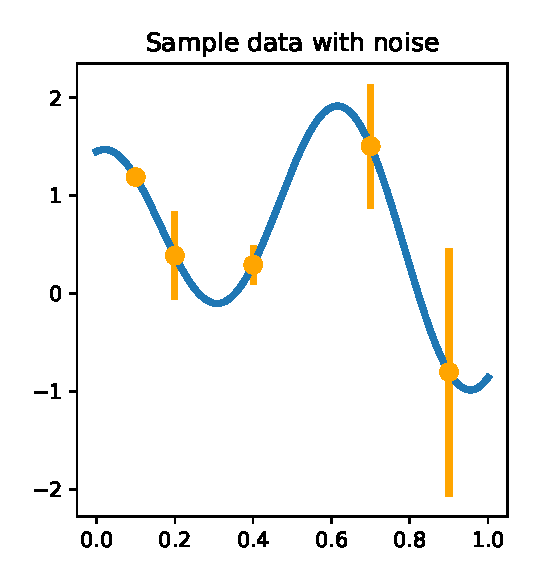
\includegraphics[height = 5cm]{ProgramsImages/sample_data.eps} \quad
	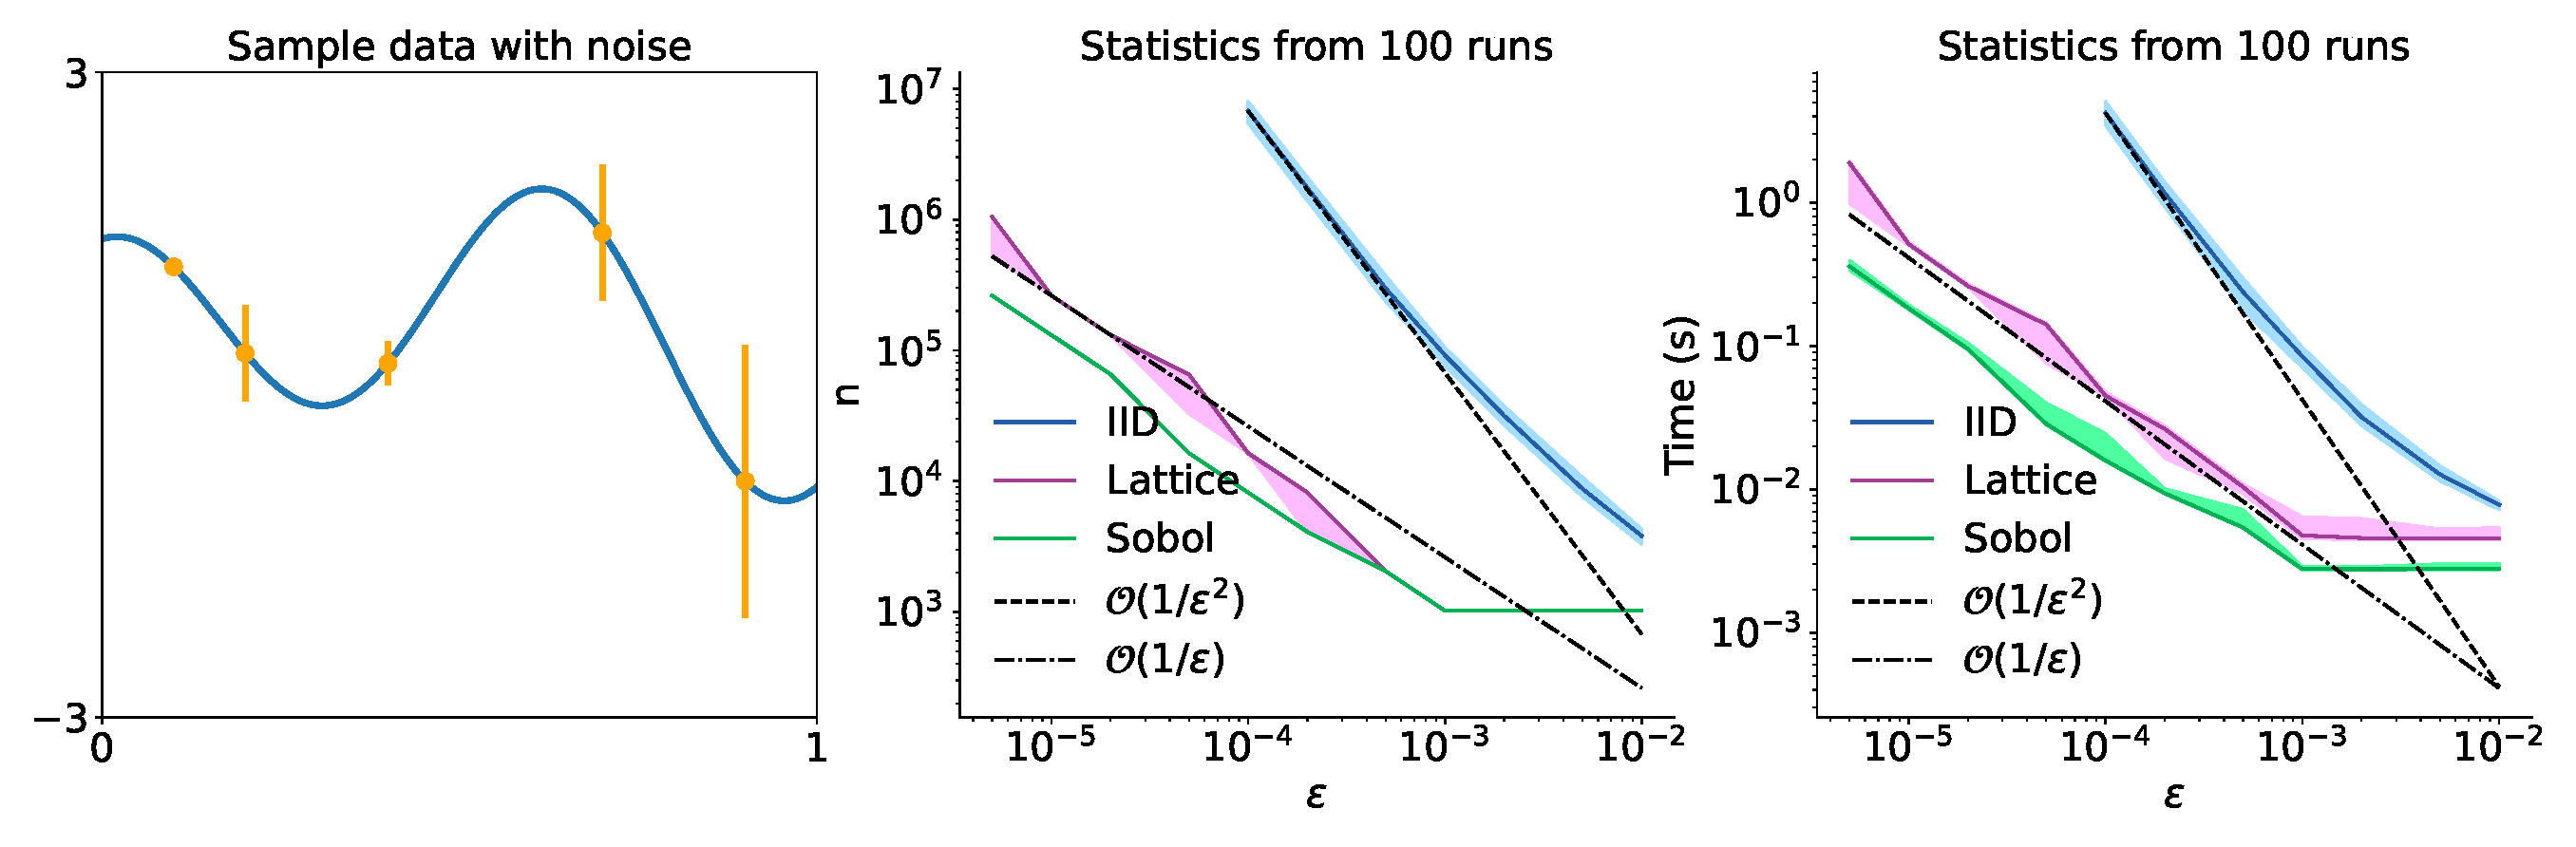
\includegraphics[height = 5cm]{ProgramsImages/qEI_cost_comp_time.eps}
	%
\includegraphics[height = 5cm]{ProgramsImages/qEI_cost_comp_n.eps} 
	\caption{Number of function values (left) and run time (right) required to compute the Keister integral \eqref{eq:Keister} using QMCPy.  LD sampling is much more efficient than IID sampling, especially as the error tolerance decreases.}
	\label{fig:qei}
\end{figure}

QMCPy as an aggregator

**parallel computing

**GPUs

MLQMC

CUD

custom LD points

Plug and play nets

more use cases

alternatives to discrepancy

Sobol' indices

higher order nets

%quantiles

**kernel density estimation
\iffalse
Pierre L'Ecuyer's talk
https://media.ed.ac.uk/playlist/dedicated/51612401/1_0z0wec2z/1_r1x3xmle

https://drive.google.com/file/d/1uztn18UimvdIo3hyYXywUaOxj_wqPJ7N/edit

\fi

SM **sampling from large data
  Thinning samples
  
SM Bayesian inference ??

SM importance sampling/control variates

\iffalse
https://media.ed.ac.uk/playlist/dedicated/51612401/1_0z0wec2z/1_jkdkrau0

https://drive.google.com/file/d/1UfZinskltBhhAQcYFAzf26FIPFje5aM-/edit

\fi



\section{Results from NSF Support} \label{sec:prior_work}

\subsection{NSF-DMS-1522687\except{toc}{, \emph{Stable, Efficient, Adaptive Algorithms for 
			Approximation and Integration},
		\$270,000, August 2015 -- July 2018}
} \label{sec:Previous}
%%%%%%%%%%%%%%%%%%%%%%%%%%%%%%%%%%%%%%%%%%%%%%%%%%%%%%%%%%%%%%%%%%%%%%%%%%%%%%%%%%%

Gregory E.\ Fasshauer (GEF, co-PI) and FH (PI) led this project, and SCTC contributed as senior personnel.  Other major contributors were FH's research students Yuhan Ding (YD, PhD 2015), Lan Jiang (LJ, PhD 2016), 
Llu\'is Antoni Jim\'enez Rugama (LlAJR, PhD 2016), Da Li (DL, MS 2016), Jiazhen Liu (JL, MS 2018), Jagadeeswaran Rathinavel (JR, 
PhD 2019), Xin Tong (XT, MS 2014, PhD 2020 @ University of Illinois at Chicago), Kan Zhang (KZ, PhD student), Yizhi Zhang (YZ, PhD 2018), and Xuan Zhou (XZ, PhD 2015).  Articles, theses,  
software, and preprints supported in 
part by this 
grant 
include 
\cite{ala_augmented_2017, 
	ChoEtal17a,
	ChoEtal19a,
	Din15a, 
	DinHic20a,
	GilEtal16a,
	Hic17a,
	HicJag18b,
	HicJim16a,
	HicEtal18a,
	HicEtal17a,
	HicKriWoz19a,
	RatHic19a,
	GilJim16b,
	JimHic16a,
	JohFasHic18a,
	Li16a,
	Liu17a,
	MarEtal18a,
	mccourt_stable_2017,
	MCCEtal19a,
	mishra_hybrid_2018,
	MisEtal19a,
	rashidinia_stable_2016,
	rashidinia_stable_2018,
	Zha18a,
	Zha17a,
	Zho15a,
	ZhoHic15a}.

%%%%%%%%%%%%%%%%%%%%%%%%%%%%%%%%%%%%%%%%%%%%%%%%%%%%%%%%%%%%%%%%%%%%%%%%%%%%%%%%%%%
\subsubsection{Intellectual Merit from Previous NSF Funding}
\label{previousmeritsubsec}
%%%%%%%%%%%%%%%%%%%%%%%%%%%%%%%%%%%%%%%%%%%%%%%%%%%%%%%%%%%%%%%%%%%%%%%%%%%%%%%%%%%
\phantom{a}

\iffalse
\begin{wrapfigure}{r}{0.4\textwidth}
	\centering
	\vspace{-1ex}
	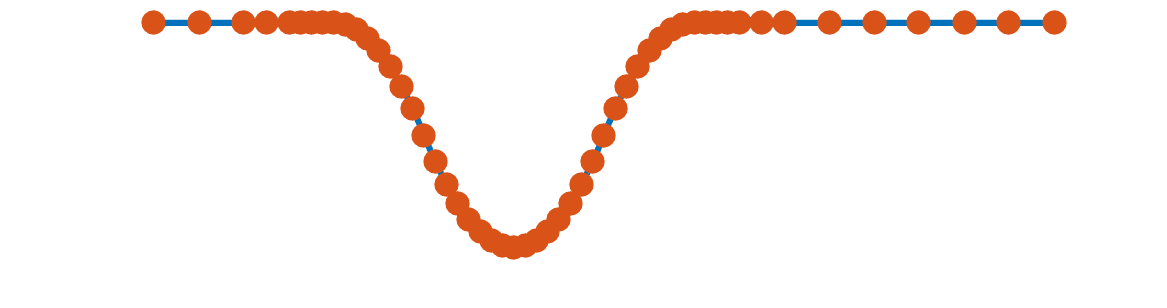
\includegraphics[width = 0.4\textwidth]{ProgramsImages/sampling-funappxg.png}
	\\
	
\includegraphics[width = 0.4\textwidth]{ProgramsImages/sampling-funming.png}
	
	\vspace{-2ex}
	\caption{The function data ({\color{MATLABOrange}$\bullet$}) for the locally adaptive 
		function approximation (top) and minimization (bottom) algorithms in \cite{ChoEtal17a}.  Sampling is denser where $\abs{f''}$ is larger.  For minimization it is also denser where the function values are smaller. \label{localadaptfig}}
\end{wrapfigure}
\fi

%%%%%%%%%%%%%%%%%%%%%%%%%%%%%%%%%%%%%%%%%%%%%%%%%%%%%%%%%%%%%%%%%%%%%%%%%%%%%%%%%%%
\paragraph{Adaptive Algorithms for Univariate Problems} \label{sec:localadpat}
%%%%%%%%%%%%%%%%%%%%%%%%%%%%%%%%%%%%%%%%%%%%%%%%%%%%%%%%%%%%%%%%%%%%%%%%%%%%%%%%%%%
FH, STSC, YD, XT, YZ and collaborators developed several adaptive algorithms for univariate integration, function approximation, and optimization \cite{ChoEtal17a,HicEtal14b,  Din15a, Ton14a, Zha18a}.  Most of these algorithms are \emph{globally adaptive}---the sampling density is constant. However, the function approximation and integration algorithms constructed by FH, SCTC, YD, and XT in \cite{ChoEtal17a} are \emph{locally adaptive}, meaning that the sampling density is non-uniform and influenced by the function data.  For function approximation, the adaptive sample is denser where $\abs{f''}$ is larger.  This locally adaptive function approximation algorithm has a computational cost of $\Order\left(\sqrt{\norm[1/2]{f''}/\varepsilon} \right)$, where $\varepsilon$ is the error tolerance, and is essentially optimal.  An intriguing aspect is the appearance of the $1/2$-quasinorm $\norm[1/2]{f''}$, which may be much smaller than 
$\norm[\infty]{f''}$ for peaky functions.



%%%%%%%%%%%%%%%%%%%%%%%%%%%%%%%%%%%%%%%%%%%%%%%%%%%%%%%%%%%%%%%%%%%%%%%%%%%%%%%%%%%
\paragraph{Globally Adaptive Cubature Based on LD Sequences} \hypertarget{QMClink}{}
\label{sec:QMC}
%%%%%%%%%%%%%%%%%%%%%%%%%%%%%%%%%%%%%%%%%%%%%%%%%%%%%%%%%%%%%%%%%%%%%%%%%%%%%%%%%%%
FH, LlAJR, DL, and JR developed globally adaptive algorithms for approximating $d$-dimensional integrals,  $\int_{[0,1]^d} f(\bx) \, \dif \bx$, based on LD sequences \cite{HicJim16a,HicEtal17a,JimHic16a}.  After the conclusion of this project, these stopping criteria are implemented in QMCPy. Two common LD sequences are integration lattice nodes and digital sequences \cite{DicEtal14a}, LD .  The error bounds underlying the adaptive cubatures developed by FH, LlAJR, DL are based on tracking the  Fourier coefficients of the sampled function values on these LD sequences.  FH and JR base their automatic Bayesian cubature on credible intervals, where the hyper-parameters of the priors are treated by empirical Bayes (maximum likelihood estimation), full Bayes, and/or cross-validation.   FH and JR chose covariance kernels that matched the LD sequences and reduced the computational cost to $\Order(n \log(n))$, making Bayesian cubature practical. 

%%%%%%%%%%%%%%%%%%%%%%%%%%%%%%%%%%%%%%%%%%%%%%%%%%%%%%%%%%%%%%%%%%%%%%%%%%%%%%%%%%%
\paragraph{Multivariate Function Approximation} \label{sec:PrevFunAppx}
%%%%%%%%%%%%%%%%%%%%%%%%%%%%%%%%%%%%%%%%%%%%%%%%%%%%%%%%%%%%%%%%%%%%%%%%%%%%%%%%%%%
FH, YD, and LlAJR and collaborators investigated function approximation problems for Banach spaces, $\calf$, defined by general series representations \cite{DinHic20a,DinEtal20a}.  For example, the bases can be general multivariate polynomials.  Three different definitions of cone, $\calc$, of functions were defined, all describing a reasonable behavior of the series coefficients.  Adaptive function approximation algorithms were constructed for these three cones shown to be essentially optimal.  The shortcoming of this research is that the algorithms use series coefficients as data rather than function values. 


%%%%%%%%%%%%%%%%%%%%%%%%%%%%%%%%%%%%%%%%%%%%%%%%%%%%%%%%%%%%%%%%%%%%%%%%%%%%%%%%%%%
\subsubsection{Broader Impacts from Previous NSF Funding} \label{prevBIsect}
%%%%%%%%%%%%%%%%%%%%%%%%%%%%%%%%%%%%%%%%%%%%%%%%%%%%%%%%%%%%%%%%%%%%%%%%%%%%%%%%%%%
\phantom{a}

\Upara{Publications, Conference Participation, Conference Organization, and Leadership} Publications by GEF, FH,  SCTC, students, and collaborators are listed at the beginning of this section.  We have spoken at many applied mathematics, statistics, 
and computational science conferences and given colloquium/seminar talks to mathematics and 
statistics departments.  FH co-organized the 
2016 Spring Research 
Conference, a long-running annual industrial statistics conference.   FH gave an invited tutorial
at MCQMC 2016
\cite{Hic17a}, a biennial conference for which he serves on the steering committee.  FH 
was a program leader for the SAMSI 2017--18 Quasi-Monte Carlo (QMC) Program.   FH received the 2016 Joseph F.\ Traub Prize for Achievement in Information-Based Complexity. In recognition of his research leadership, FH was appointed the director of Illinois Tech's new Center for Interdisciplinary 
Scientific Computation in 2017.  In 2018, FH was appointed Vice Provost for Research.

\Upara{\GAIL Software} The results of this research have been implemented in 
\GAIL, our open source \MATLAB library hosted on
Github. This software 
has been implemented with input parsing, input validation, unit tests, inline documentation, and 
demonstrations.  \GAIL makes it easier for practitioners to try our new adaptive algorithms.  SCTC has been key in this effort.  \GAIL has been used in the yearly graduate course in Monte Carlo methods taught by FH and YD.  
%With the help of students, we are starting to port GAIL to Python and \Rlang.

\Upara{Boosting the STEM Workforce} GEF, FH, and SCTC mentored a number of 
research students associated with this project.  Female students mentored include YD, LJ, JL, XT, and Xiaoyang Zhao (MS 2017).   GEF, FH,  and SCTC have mentored many undergraduate students including more than a dozen 
Brazilian Science Mobility Program students in the summers of 2015 and 2016, plus eight other students (two female) from Illinois Tech, Biola U, U Minnesota, Macalester U, NUS, Colorado School of Mines.  All but one have enrolled in graduate programs.   As part of our team, all of
these students have learned how to conduct theoretical and/or practical computational mathematics research.

\subsection{Simon's Results from Prior Support}

\section{Strengths of This Team and Collaboration Plan}


\subsection{Collaborations}
Prof.\ Art B. Owen (Stanford University) has engaged with the PIs in conversations about QMC for many years.  Prof.\ Owen is particularly expert in randomized QMC and the use of low discrepancy points for Markov chain Monte Carlo.  He has taken a keen interest in QMCPy and will put forward new QMC use cases, advise on software features to be included, and possibly collaborate on joint publications with the PIs.  Prof.\ Owen will also encourage his student to help out with the implementation of Sobol' indices.

Dr.\ Mike McCourt (SigOpt) convinced his company to fund the early development of QMCPy.  He was convinced of the advantages of low discrepancy sampling and wanted to spread these ideas to the tech industry.  During the first year of QMCPy's development, Mike advised us what we should prioritize for the benefit of tech practitioners.  Although SigOpt is not in a position to  fund SigOpt further, Mike will advise us on the continued development of SigOpt.  He will also help us spread the word among his network in the machine learning community.

Dr.\ Tim Sullivan (University of Warwick, UK) provides expertise on two application domains for the QMC software developed in this project.  The first area is probabilistic numerics, a Bayesian statistical approach to numerical tasks such as quadrature and the solution of differential equations, in which the solution object is a statistical posterior distribution over the value of the integral or solution to the differential equation and reflects the discretisation uncertainty inherited from the finite computational budget.  QMC methods offer an attractive way to interrogate these PN distributions at significantly lower cost than traditional MC or MCMC sampling.  The second are is the use of QMC methods in the training of metamodels for heterogeneous (i.e. mixed atomistic-continuum) systems, which is an area of particular interest in Warwick's EPSRC Centre for Doctoral Training in Modelling of Heterogeneous Systems (HetSys).

\section{Broader Impacts}

Proper handling of LD sequences 

Educating a wider user base

Branching into new applications

those who

QMCPy is proving ground


\newpage
\clearpage
%\pagenumbering{arabic}
\setcounter{page}{1}
%\renewcommand{\thepage}{D-\arabic{page}}

\bibliographystyle{spbasic}


{\renewcommand\addcontentsline[3]{} 
\renewcommand{\refname}{{\Large\textbf{References Cited}}}                   %%
\renewcommand{\bibliofont}{\normalsize}

\bibliography{FJH23,FJHown23}}
\end{document}
